
\begin{multicols*}{2}

\section{Elementalist}

\lettrine[lines=3, lhang=0.15, loversize=0.25, findent=.5em]{E}{lementalists} are multi-faceted spellcasters that channel elemental forces, making fire, earth, and lightning do their bidding. What they lack in physical toughness, they make up in versatility summoning shamanic totems to ward allies and also conjuring extremely destructive and raw magic.

\subsection*{Elemental Ward}

Twice per combat, when you or a creature within 30 feet of you takes acid, cold, fire, lightning, or thunder damage, you can use your reaction to grant resistance to the creature against that instance of the damage.

Additional uses of this class feature require spending mana points.

\subsection*{Shaman Training}

You gain proficiency with light armor and shields.

\subsection*{Shamanic Magic}

At 3rd level, you gain the ability to tap into the raw energy of the primordials. Refer to the Elementalist's shaman magic table for details.

Your shamanic magic requires you to summon a totem (no action required) embedded with the power of a single element. Treat the totem as a small creature that appears in an unoccupied space on a horizontal surface within 5 feet of you.

Until the end of your next turn, you can take a bonus action to cause the totem to activate if you are within 60 feet of it. As part of the same bonus action, you can direct the totem to slowly fly up to 20 feet to an unoccupied space near the ground. While the totem has fly speed, it hovers just above the ground unless said otherwise.
Elemental
The totem has an AC of 18 and a number of hit points equal to 4 times your level. It is immune to poison damage, psychic damage, and all conditions. If it is forced to make an ability check or saving throw, treat all it's ability scores as 10 (+0). 


\subsection*{Bend Elements}

At 5th level, you have learned how to absorb part of any income elemental damage into elemental power.

Once per round, if you take 10 or more acid, cold, fire, lightning, or thunder damage, you can spend your reaction to gain a mana point.

\subsection*{Storm, Earth, and Fire}

At 9th level, you have learned to bend and combine elements in unspeakable ways.

Blazing orbs of fire plummet to the ground, lightning strikes, and earth is torn asunder. As an action, choose three points in sight. Each creature in a 20-foot-radius sphere centred on each point takes 3d10 of fire damage, 3d10 of bludgeoning damage, and 3d10 of lightning damage.
Each affected creature must make a Dexterity and Wisdom saving throws.


On a failed Dexterity save, a creature is knocked prone and it is restrained by the debris until the start of your next turn.

On a failed Wisdom save, a creature is frightened. It must spend its next turn trying to move as far away from you as it can, and it can't willingly move to a space within 30 feet of you.

You can use this class feature once per long rest. 
You can use it two other times before a long rest. 

\begin{itemize}
    \item The first time requires you to spend 3 mana points. 
    \item The second, 4 mana points.
\end{itemize}

\begin{Figure}
\centering
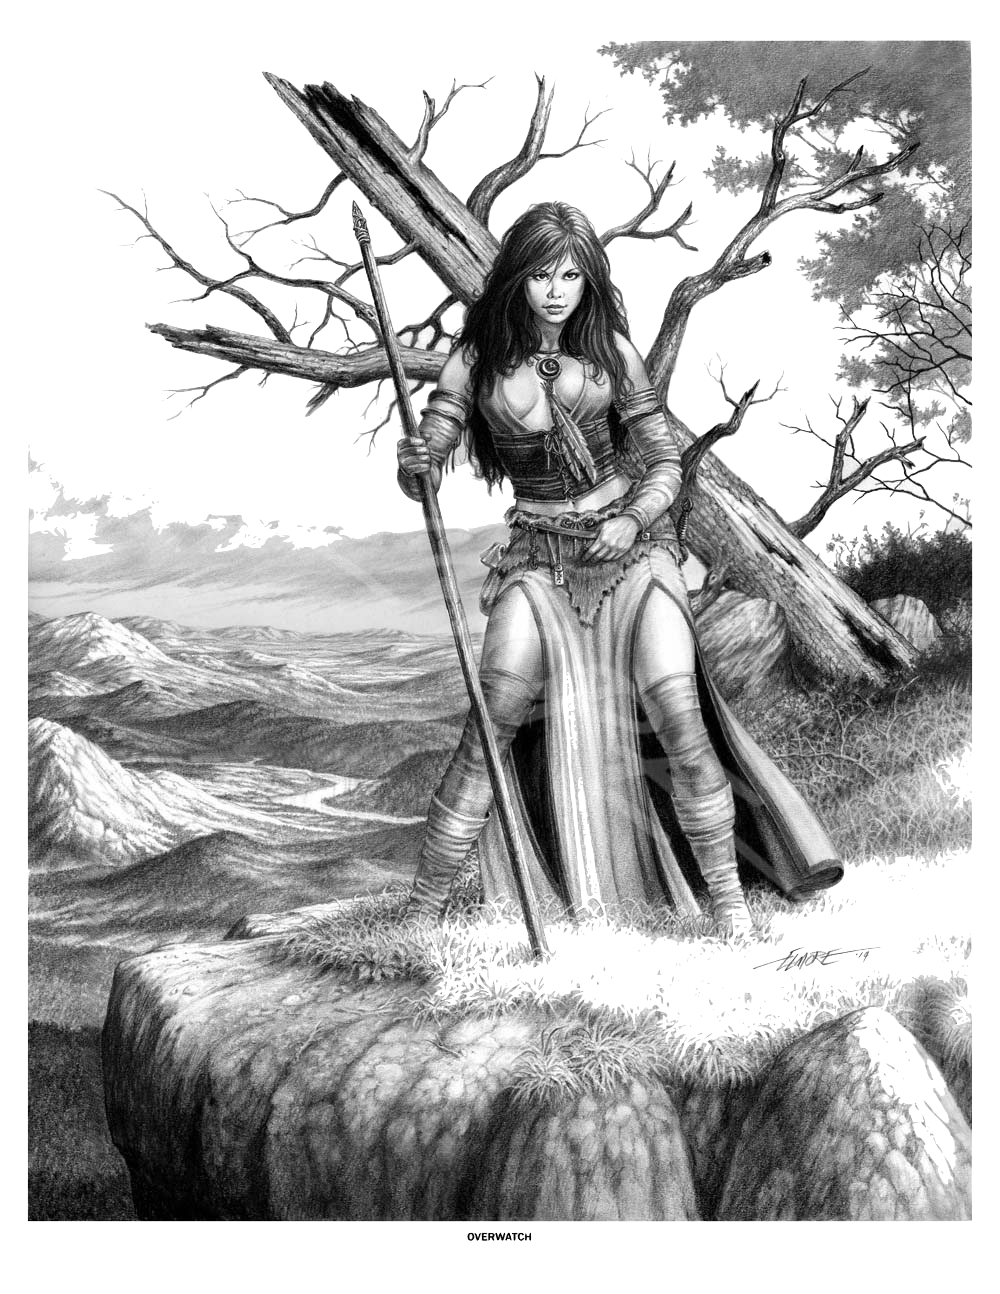
\includegraphics[width=\textwidth]{img/druid-2.png}
\end{Figure}
    
\end{multicols*}


\clearpage

\begin{table}[ht!]
\begin{small}
\rowcolors{2}{}{commentgreen}
\begin{center}
\begin{tabular}{ll}
\multicolumn{2}{l}{\parbox[l][0.6cm][c]{15cm}{\textbf{Shamanic Magic}}} 
\\
\hline 
\textbf{Name} & \parbox[l][0.6cm][c]{15cm}{\textbf{Description}}
\\ 
Typhoon Ward & \parbox[l][2.2cm][c]{15cm}{
You can spend one mana point to create an almost invisible sphere of wind and hovering leaves. The totem emits strong winds causing disadvantage in the first ranged attacks against a creature within 10 feet of the totem. Including itself. This effect activates only once per creature per turn. This totem can fly in any direction. 
}
\\ 
Geode Armor & \parbox[l][2.2cm][c]{15cm}{
You can spend one mana point to create an orb of dust, rocks, and gravel. The totem emits a burst of positive energy that grants itself and up to two creatures of your choice within 10 feet of it a number of temporary hit points equal to you mana die. The dust barrier protects the creature from natural heat.
}
\\
Pyre Leash & \parbox[l][2.2cm][c]{15cm}{
You can spend one mana point to create a sphere of flames and cinder. The totem must hover directly 5 feet above a create. The warm flames protect the creature from natural cold. Once per round, whenever the protected creature takes melee damage, the sphere rebukes with flames. The attacking creature takes your mana die fire damage.
}
\\ 
Magnetize & \parbox[l][2.4cm][c]{15cm}{
You can spend one mana point to create an orb of dust and gravel. The earth sphere fires rock javelins upon your command. 
Make a ranged spell attack, originating from the sphere, at one creature or object within 60 feet of it. On a hit, the target takes your mana die damage + your spellcasting ability modifier force damage and it is pushed 10 feet away from the totem.
}
\\
\hline
\end{tabular}
\end{center}
\end{small}
\end{table}    


\begin{multicols*}{2}
\begin{Figure}
\centering
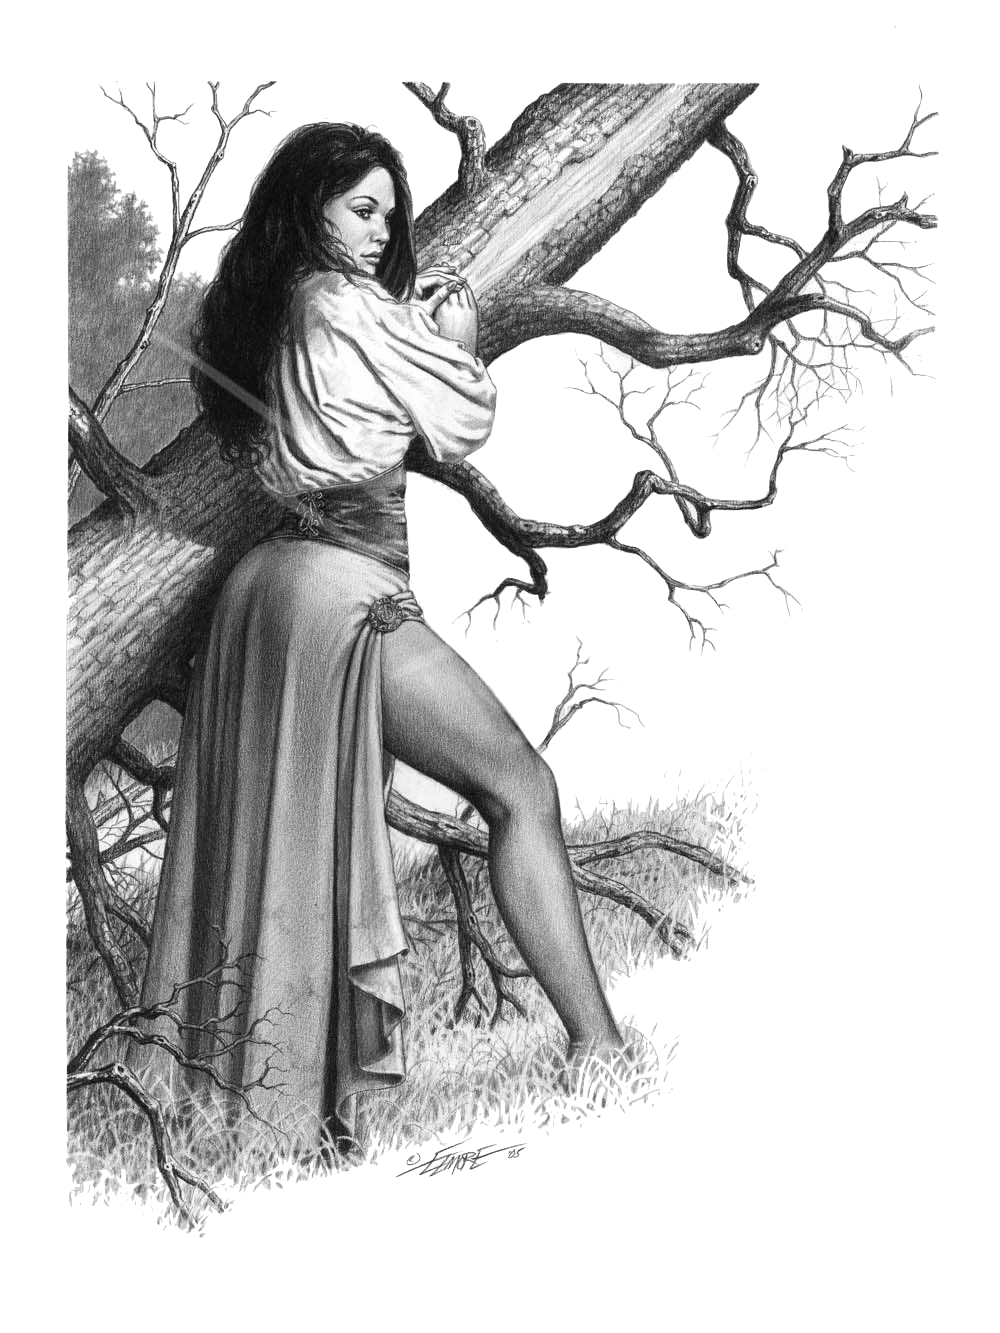
\includegraphics[width=\textwidth]{img/bard.png}
\end{Figure}
    
\end{multicols*}

        